
%% The Appendices part is started with the command \appendix;
%% appendix sections are then done as normal sections
\appendix

\section{Magnetic Field Gradient Calculations}
\label{Appendix:MagneticFieldGradientCalculations}

The maximum gradient in the z-component of the magnetic field in Figure~\ref{fig:bfield_gironeffects} was calculated by taking the difference between the maximum and the minumum magnetic-field magnitudes along the perimeter of the PMT outline (in this case in the diagonal direction), and dividing it by the distance between the two points of measurement (here, the diameter of the PMT, 20 inches = 0.508 m).
For the first plot, without any GIRON flooring, the gradient is calculated as follows:
\[[(447\pm5 \text{ mG}) - (223\pm5 \text{ mG})]/ (0.508\pm0.004 \text{ m} ) = 441\pm14 \text{ mG} \]
Similarly, the gradient for the second plot, with one layer of GIRON flooring is calculated to be $ 132\pm14 $ mG/m ($ 340\pm5 $ mG/m used as the maximum magnitude along the PMT perimeter, and $ 273\pm5 $ mG/m used as the minimum, at the opposite end of the perimeter).

The percent difference between the magnetic-field gradient with and without GIRON flooring is:
\[(132\pm14 \text{ mG})/(441\pm14 \text{ mG}) - 1 = -70.1\pm3.3 \text{ \%}\]

Therefore, a single layer of GIRON flooring helps reduce the gradient in the z-component of the magnetic field by $ 70.1\pm3.3 $ \%.

\newpage
\section{Magnetic Field Compensation Coil Configuration}
\label{Appendix:CoilPositions}
\begin{figure}[h!]
   \begin{center}
   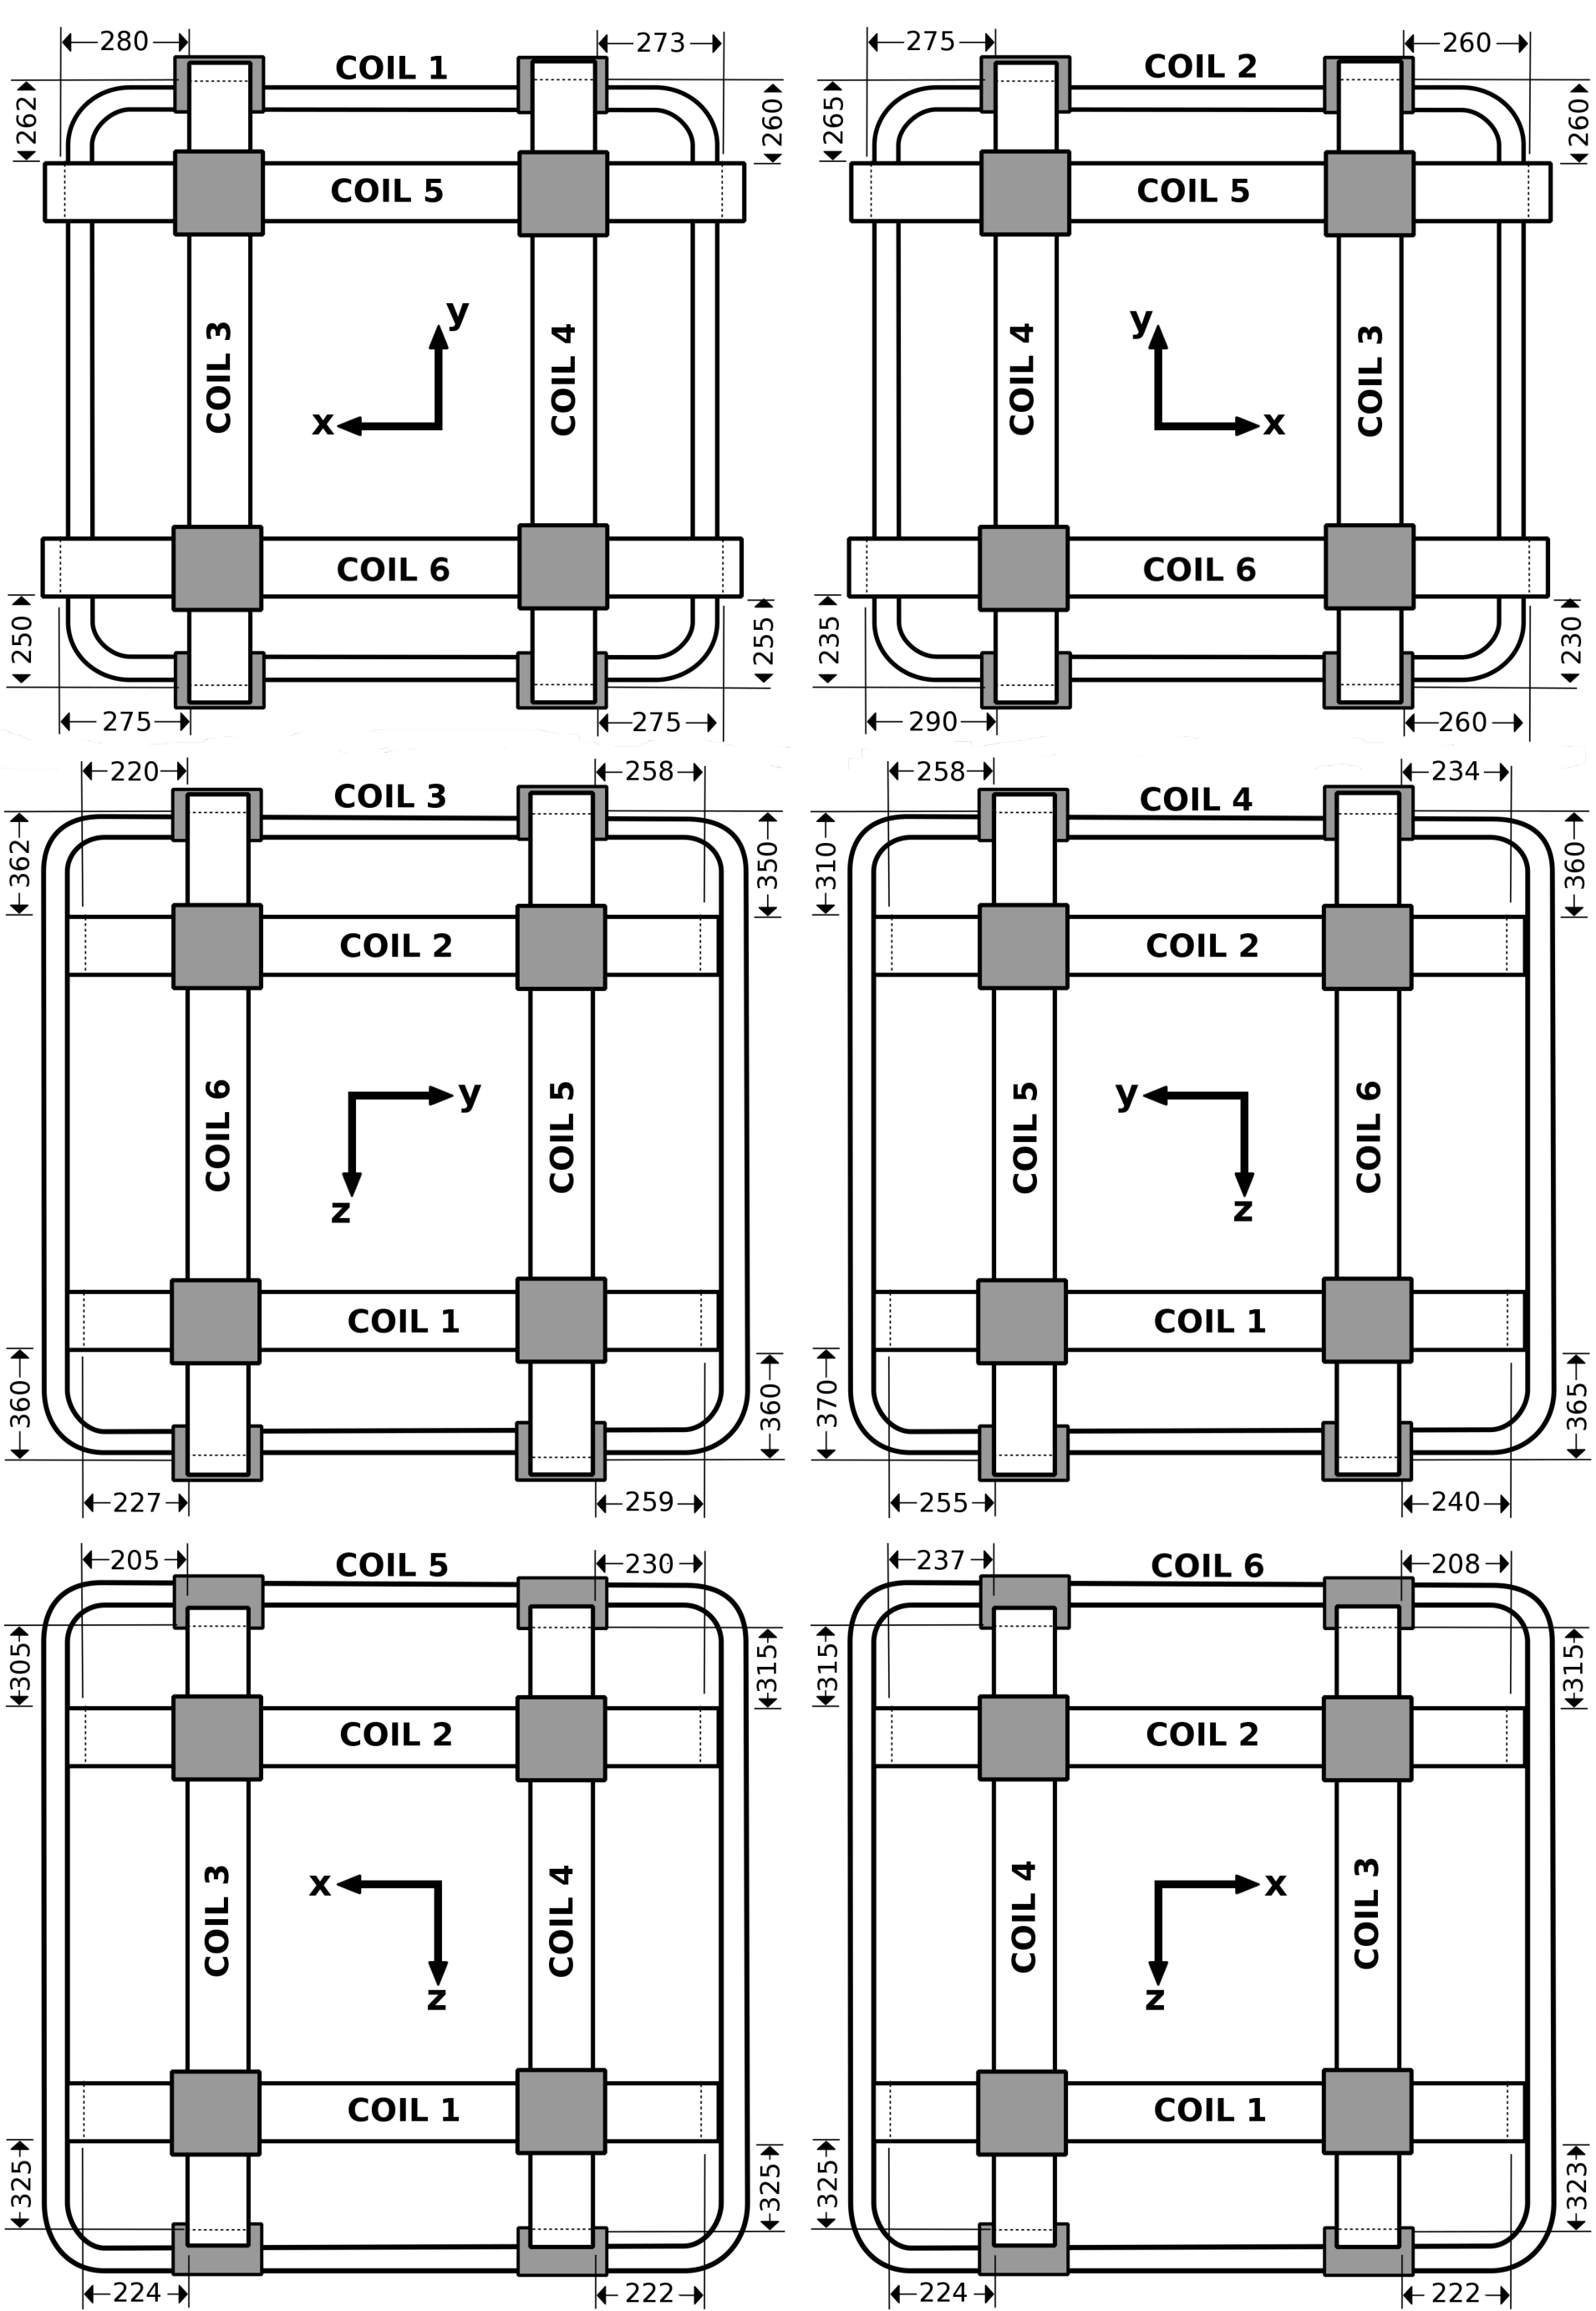
\includegraphics[width=0.7\textwidth]{bfield_PTFcoilpositions.pdf}
   \caption{PTF compensation coil positions; dimensions are in millimeters ($\pm2$ mm).}
   \label{fig:coilpos}
   \end{center}
\end{figure}

\newpage
\section{Magnetic Field Scan Plots}
\label{Appendix:MagneticFieldScanPlots}

\subsection{Fully Compensated Magnetic Field}
\label{Appendix:PlotsofFullCompensation}

The following plots show a few magnetic field maps in the x-y plane at different heights for when the magnetic field in the PTF is fully compensated, so that the center of the scan volume has a magnetic field of zero magnitude.

%
\begin{figure}[h!]
  \begin{center}
    \subfloat[Magnetic field magnitude and vector field\label{fig:bfield_fullcomp400_vec}]{
      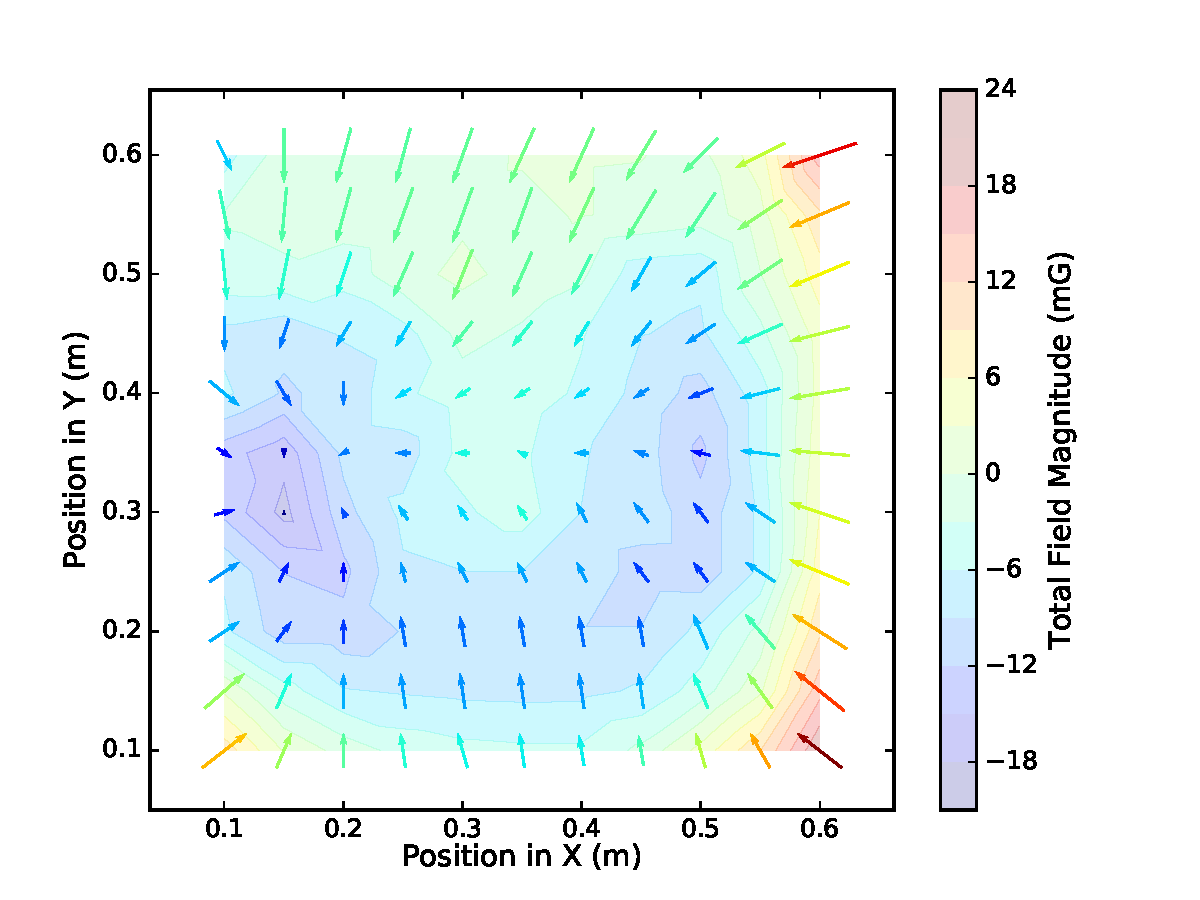
\includegraphics[width=0.5\textwidth]{bfield_full_compensation_z400_vec.pdf}
    }
    \subfloat[x-component of magnetic field\label{fig:bfield_fullcomp400_x}]{
      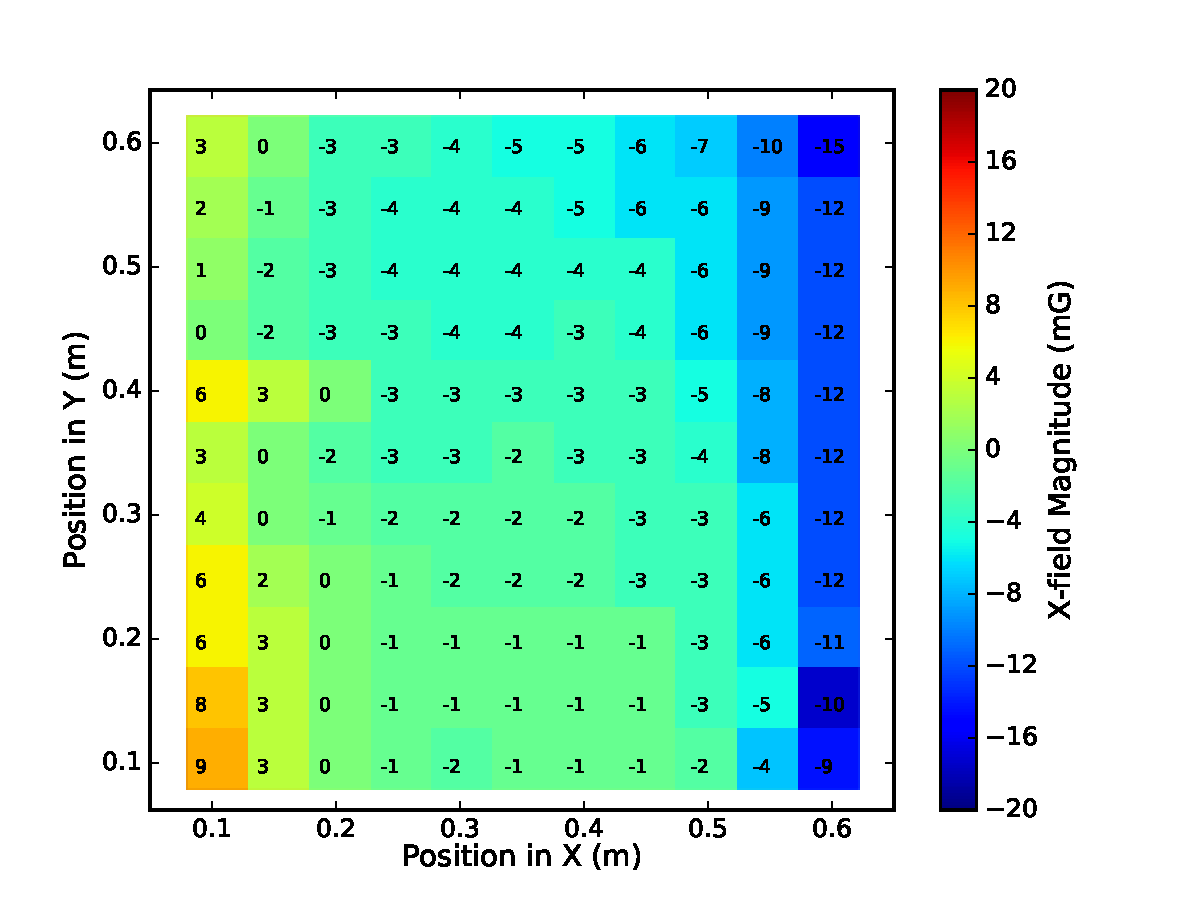
\includegraphics[width=0.5\textwidth]{bfield_full_compensation_z400_x.pdf}
    }\\
    \vspace{-3 mm}
    \subfloat[y-component of magnetic field\label{fig:bfield_fullcomp400_y}]{
      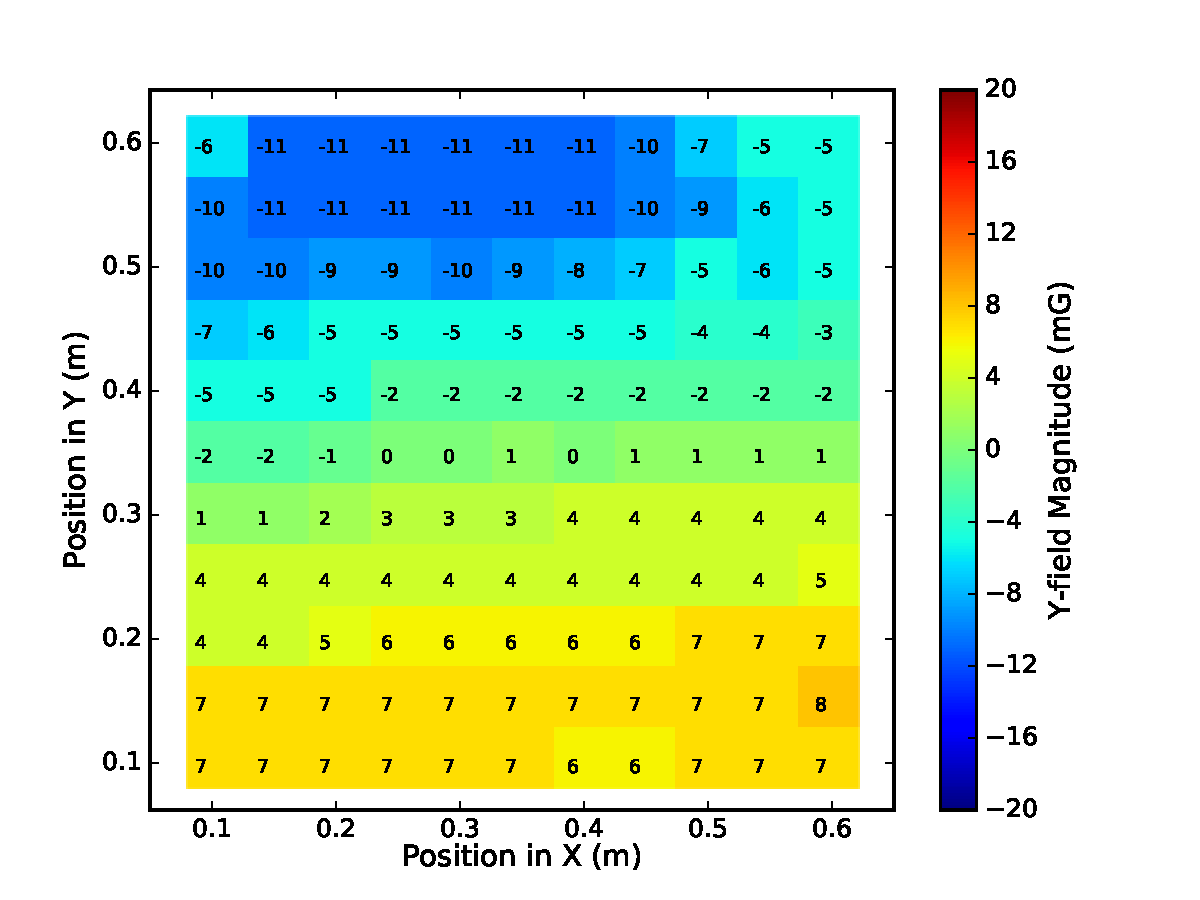
\includegraphics[width=0.5\textwidth]{bfield_full_compensation_z400_y.pdf}
    }
    \subfloat[z-component of magnetic field\label{fig:bfield_fullcomp400_z}]{
      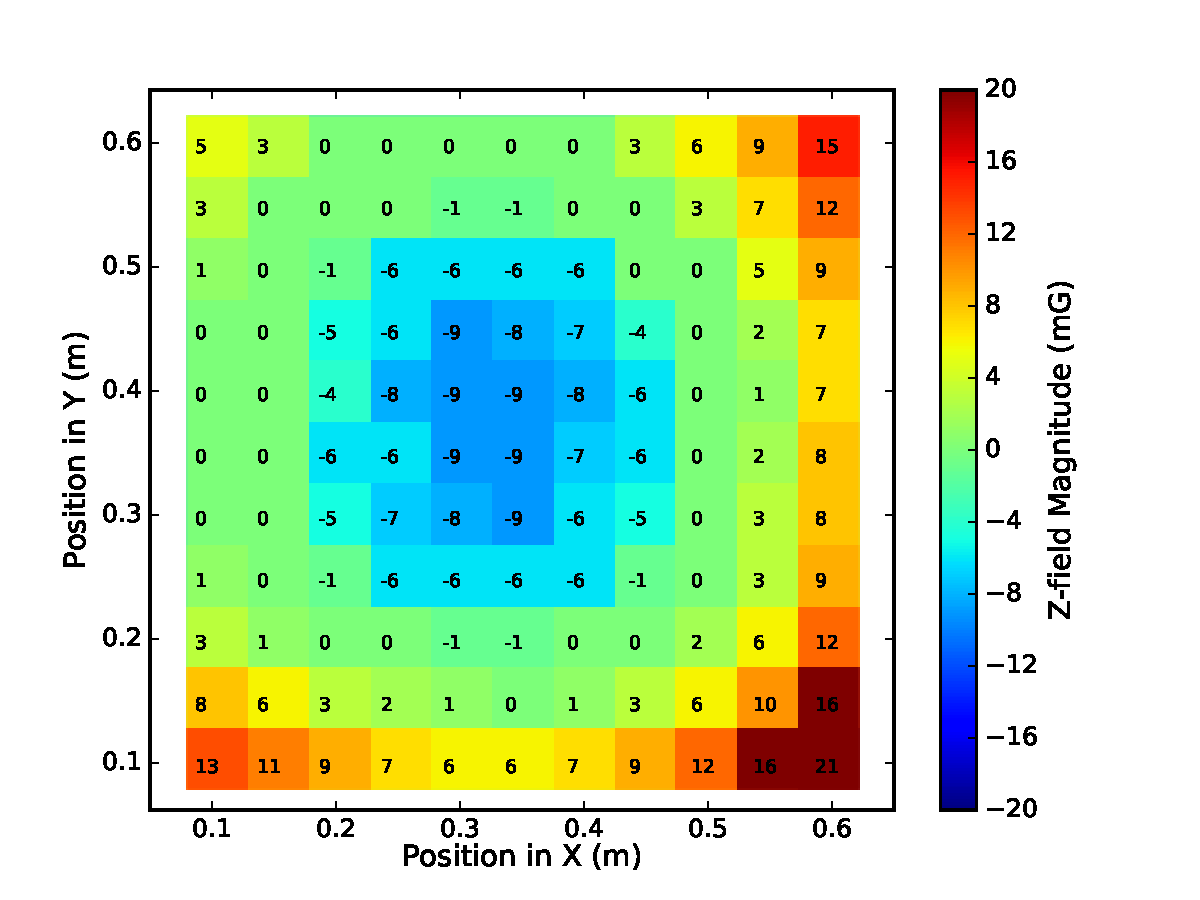
\includegraphics[width=0.5\textwidth]{bfield_full_compensation_z400_z.pdf}
    }
  \caption{Plots of fully compensated magnetic field in the x-y plane at a height just above the top of the PMT (z = 0.4 m).}
  \label{fig:bfield_fullcomp400}
  \end{center}
\end{figure}
%
%
\begin{figure}[h!]
  \begin{center}
    \subfloat[Magnetic field magnitude and vector field\label{fig:bfield_fullcomp600_vec}]{
      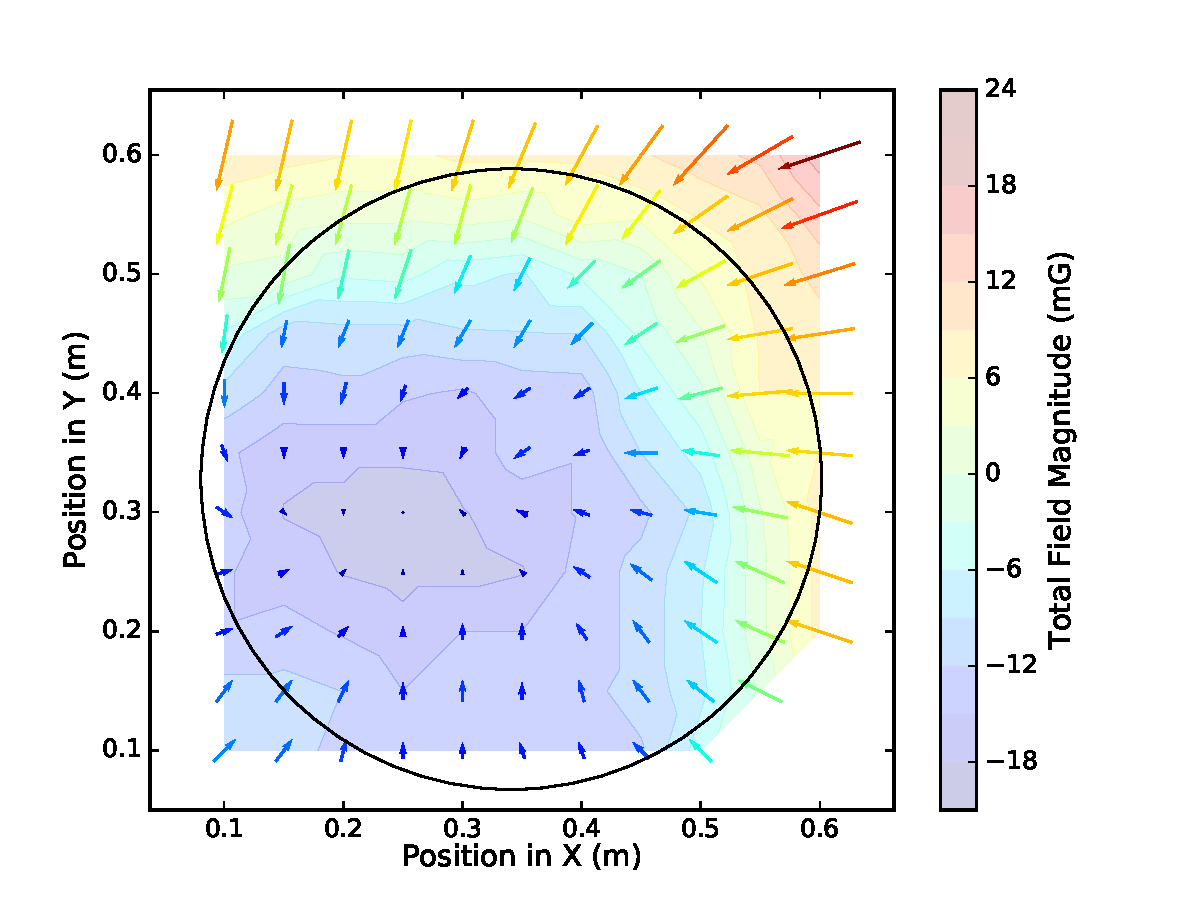
\includegraphics[width=0.5\textwidth]{bfield_full_compensation_z600_vec.pdf}
    }
    \subfloat[x-component of magnetic field\label{fig:bfield_fullcomp600_x}]{
      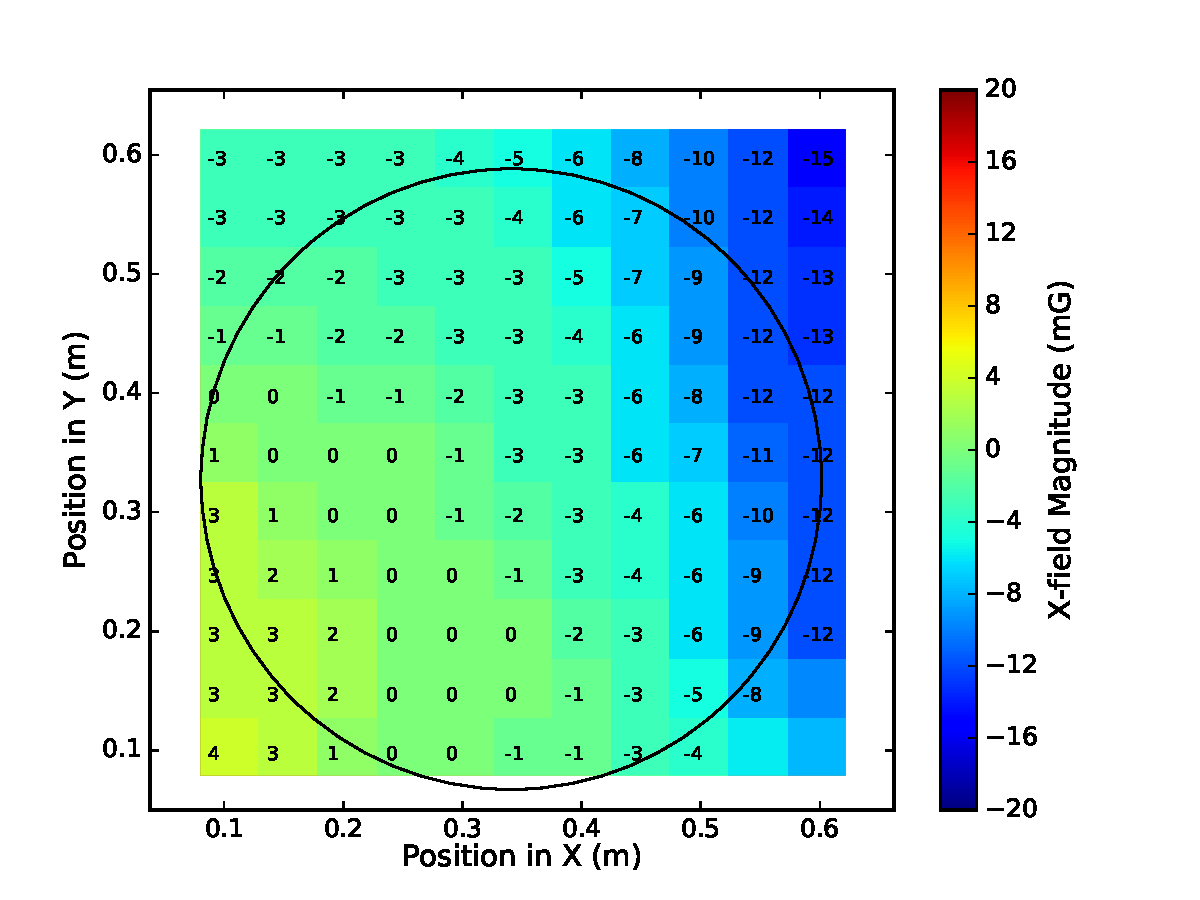
\includegraphics[width=0.5\textwidth]{bfield_full_compensation_z600_x.pdf}
    }\\
    \vspace{-3 mm}
    \subfloat[y-component of magnetic field\label{fig:bfield_fullcomp600_y}]{
      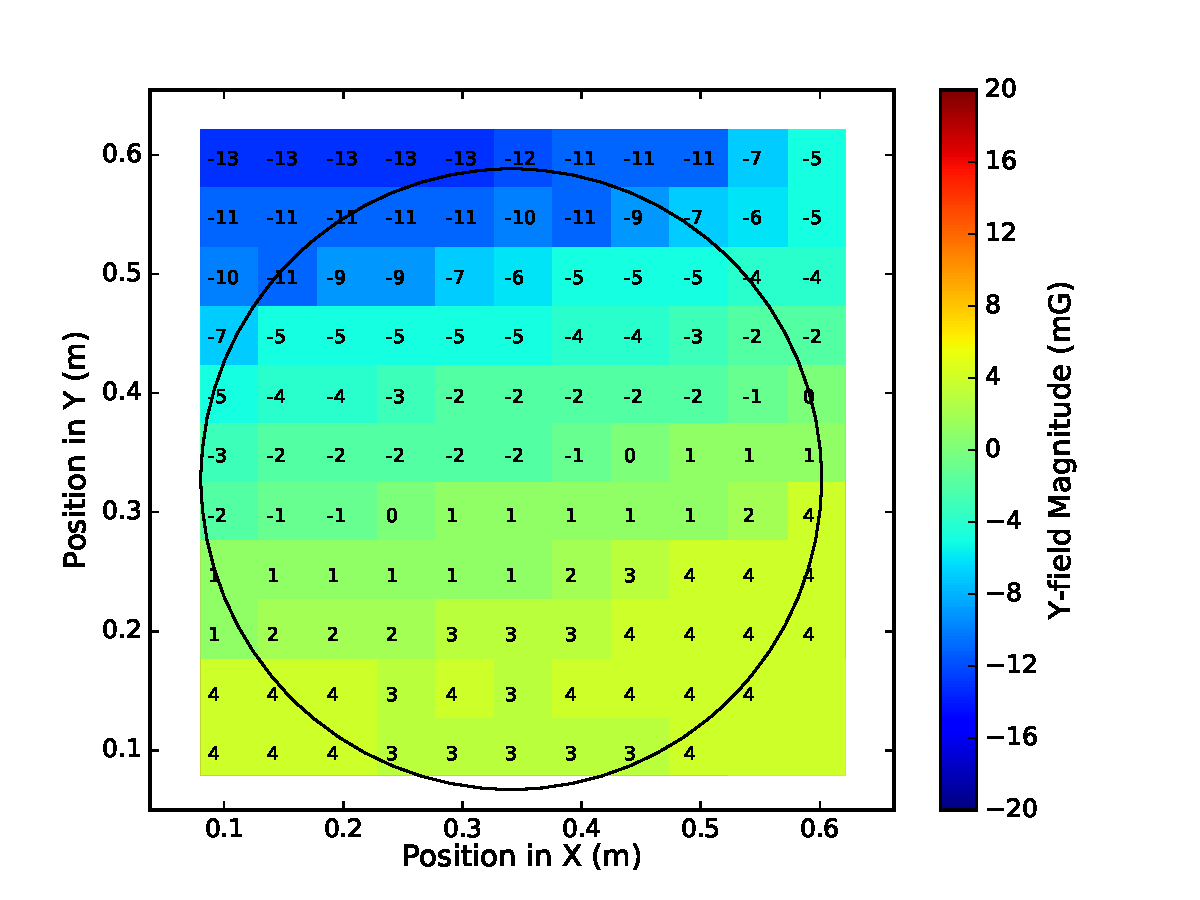
\includegraphics[width=0.5\textwidth]{bfield_full_compensation_z600_y.pdf}
    }
    \subfloat[z-component of magnetic field\label{fig:bfield_fullcomp600_z}]{
      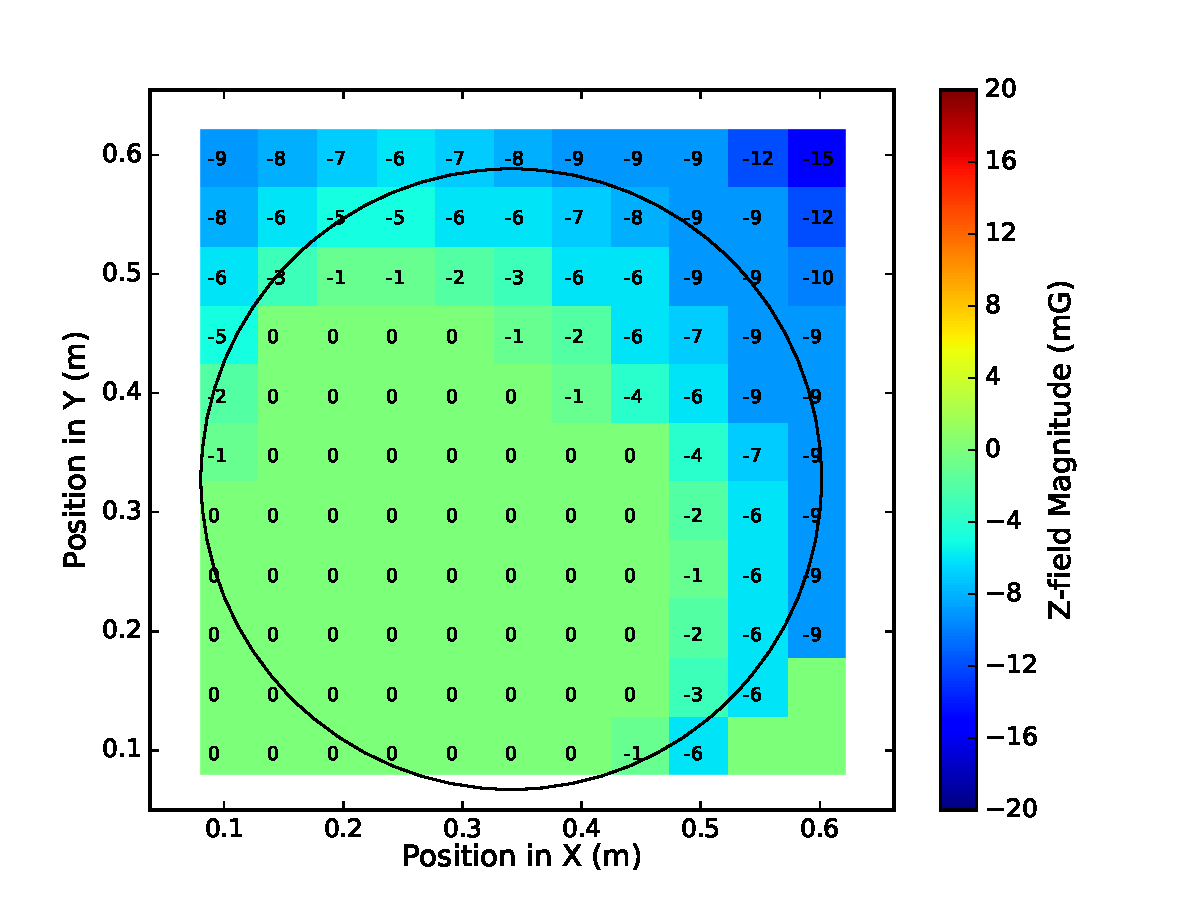
\includegraphics[width=0.5\textwidth]{bfield_full_compensation_z600_z.pdf}
    }
  \caption{Plots of fully compensated magnetic field in the x-y plane at the height of the center of the 20'' PMT's electron-path trajectory (z = 0.6 m).}
  \label{fig:bfield_fullcomp600}
  \end{center}
\end{figure}
%
%
\begin{figure}[h!]
  \begin{center}
    \subfloat[Magnetic field magnitude and vector field\label{fig:bfield_fullcomp800_vec}]{
      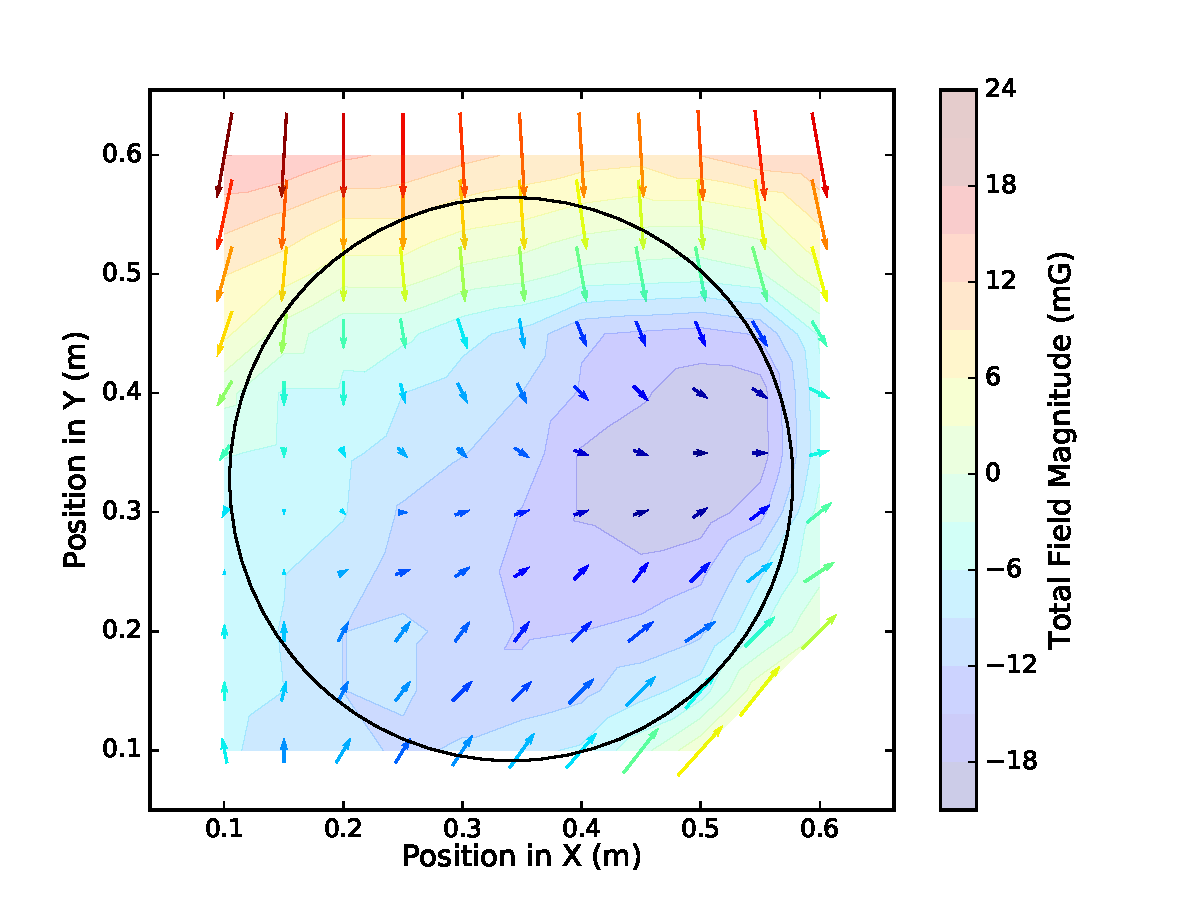
\includegraphics[width=0.5\textwidth]{bfield_full_compensation_z800_vec.pdf}
    }
    \subfloat[x-component of magnetic field\label{fig:bfield_fullcomp800_x}]{
      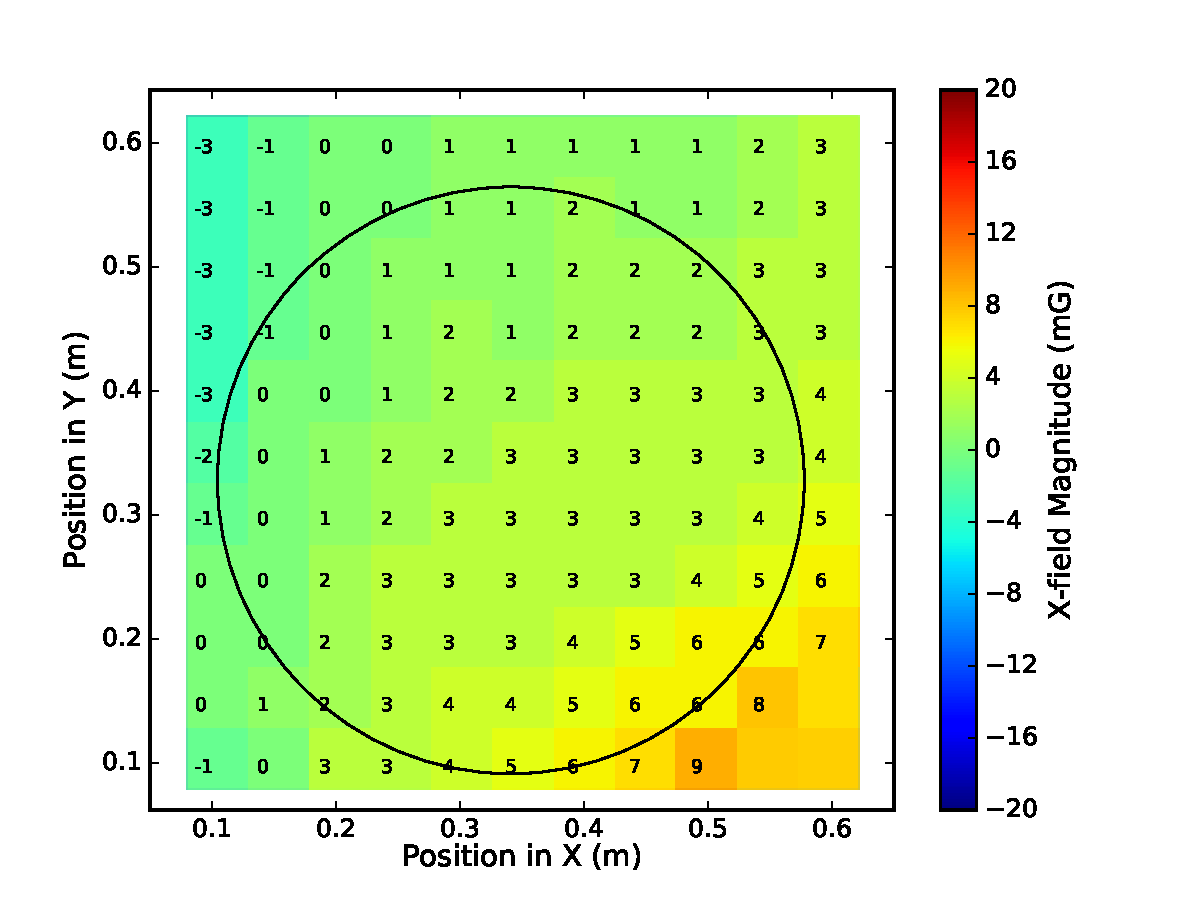
\includegraphics[width=0.5\textwidth]{bfield_full_compensation_z800_x.pdf}
    }\\
    \vspace{-3 mm}
    \subfloat[y-component of magnetic field\label{fig:bfield_fullcomp800_y}]{
      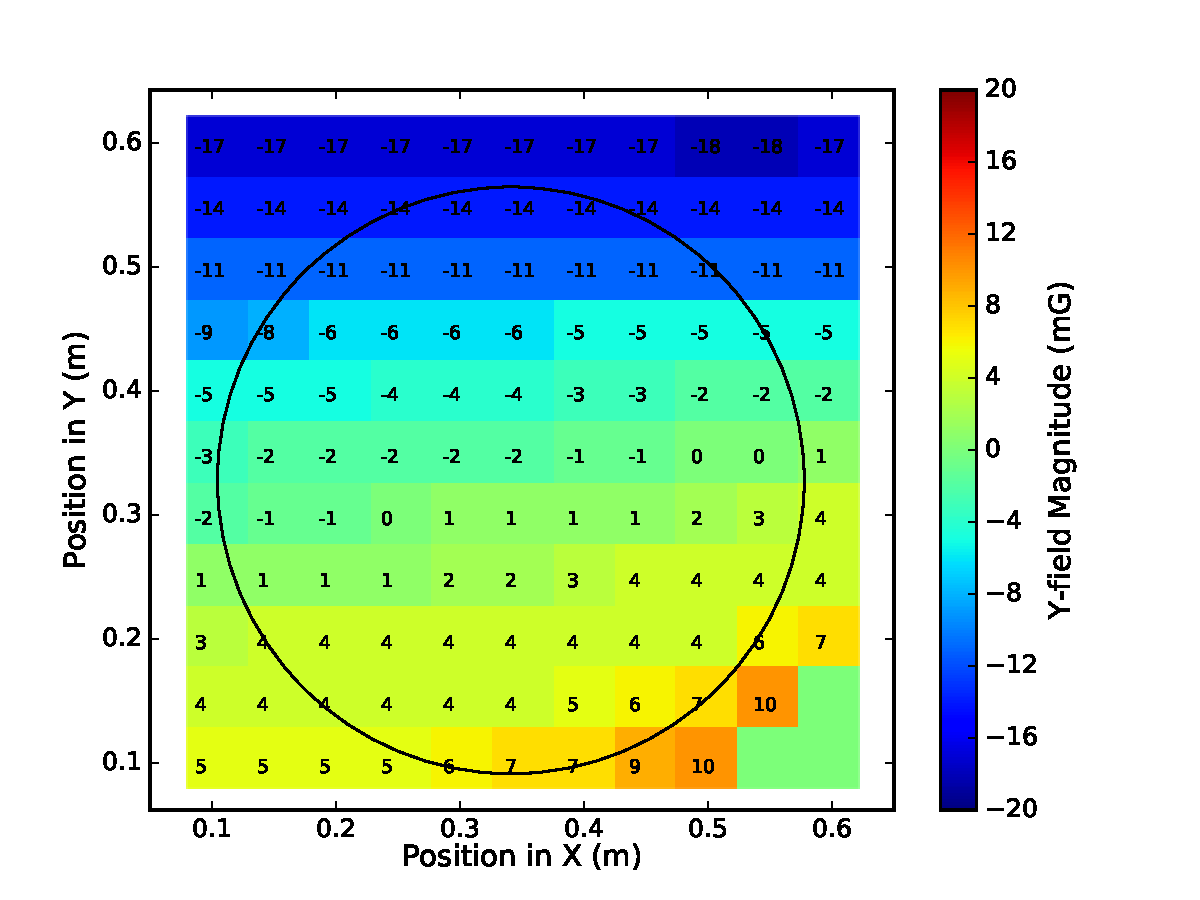
\includegraphics[width=0.5\textwidth]{bfield_full_compensation_z800_y.pdf}
    }
    \subfloat[z-component of magnetic field\label{fig:bfield_fullcomp800_z}]{
      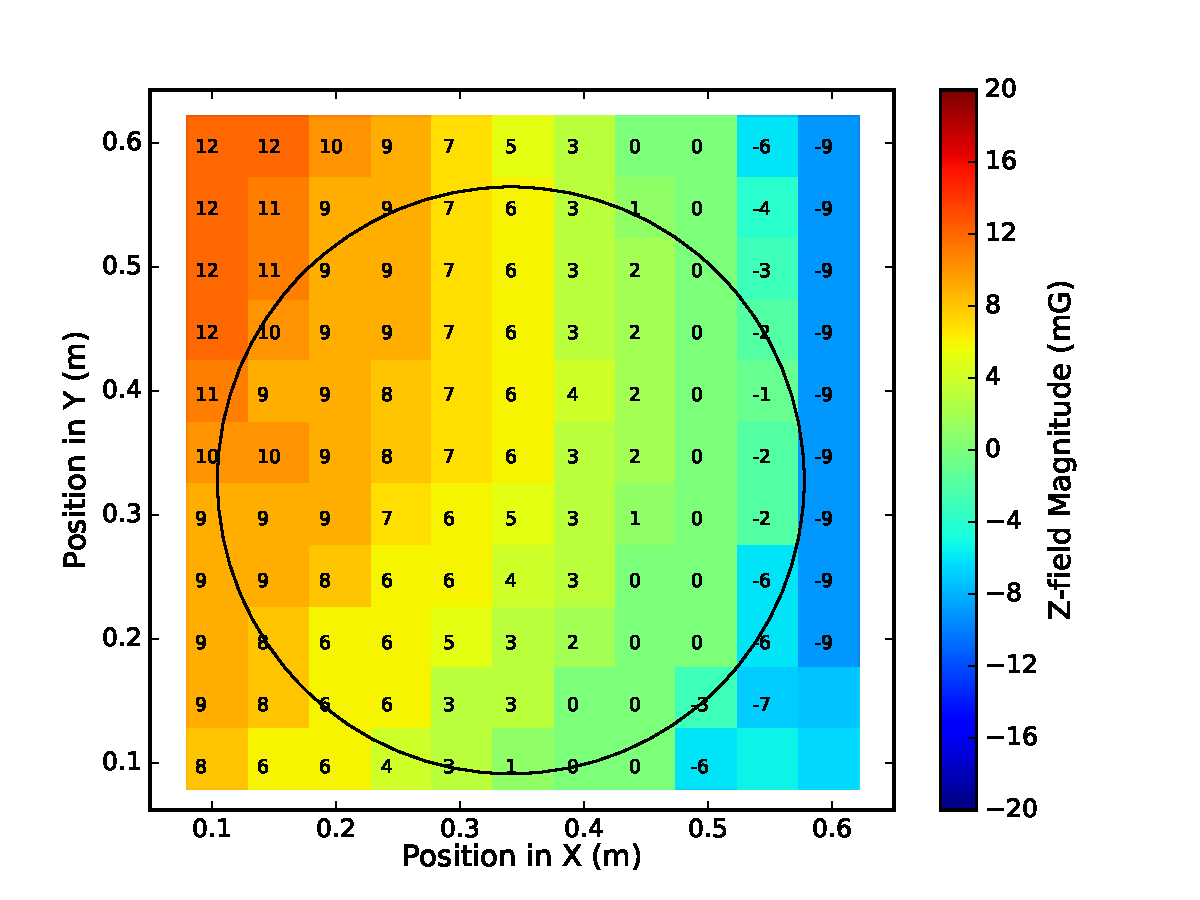
\includegraphics[width=0.5\textwidth]{bfield_full_compensation_z800_z.pdf}
    }
  \caption{Plots of fully compensated magnetic field in the x-y plane at the height of the first dynode of the 20'' PMT (z = 0.8 m).}
  \label{fig:bfield_fullcomp800}
  \end{center}
\end{figure}
%

\newpage
\subsection{Reproducibility Test}
\label{Appendix:ReproducibilityTest}

The following magnetic field maps show the accuracy to which the magnetic fields can be controlled, and the reproducibility of different magnetic field conditions.
All plots show the magnetic fields mapped in the x-y plane at the height of the center of the electron path trajectory.

%
\begin{figure}[h!]
  \begin{center}
    \subfloat[Trial 1: magnetic field magnitude and vector field\label{fig:bfield_rep_Bx50_1_vec}]{
      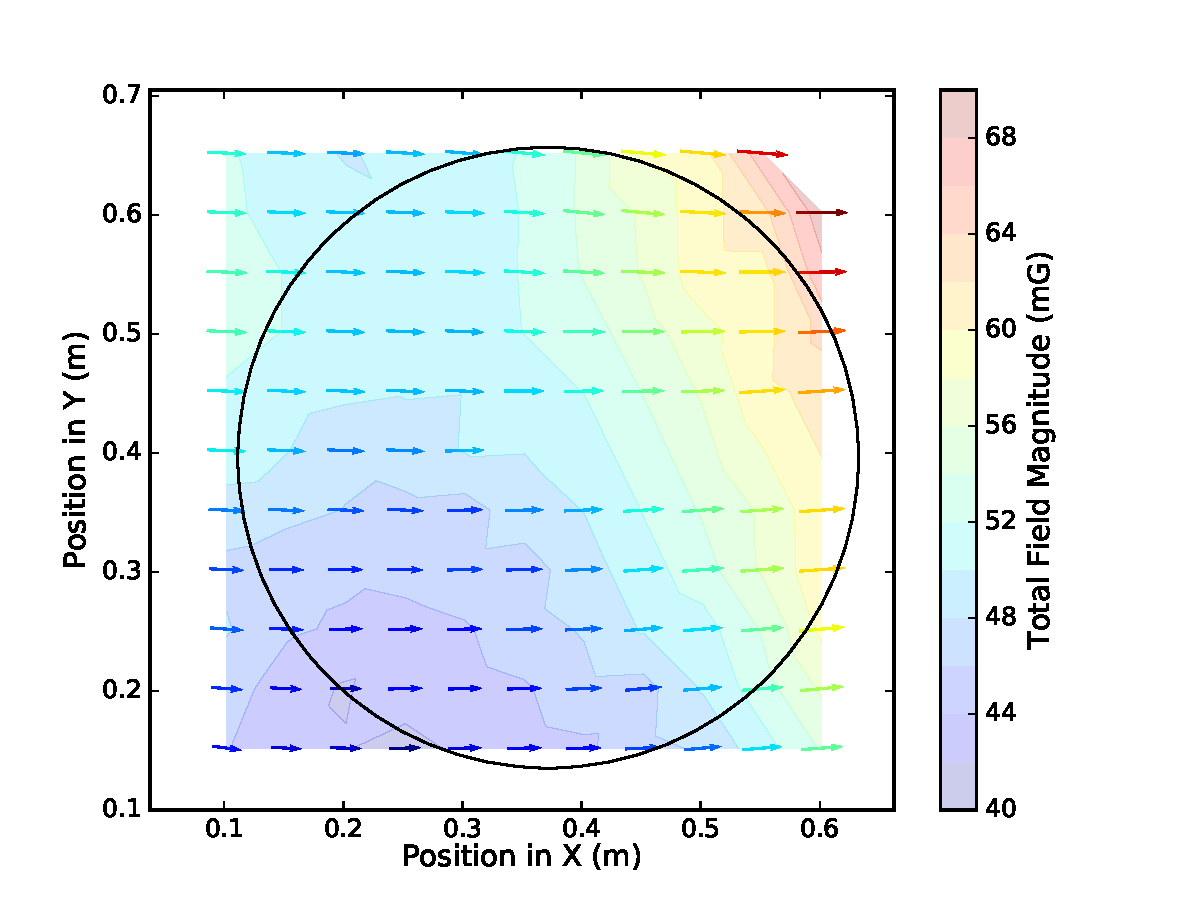
\includegraphics[width=0.5\textwidth]{bfield_rep_Bx50_z700_1_vec.pdf}
    }
    \subfloat[Trial 2: magnetic field magnitude and vector field\label{fig:bfield_rep_Bx50_2_vec}]{
      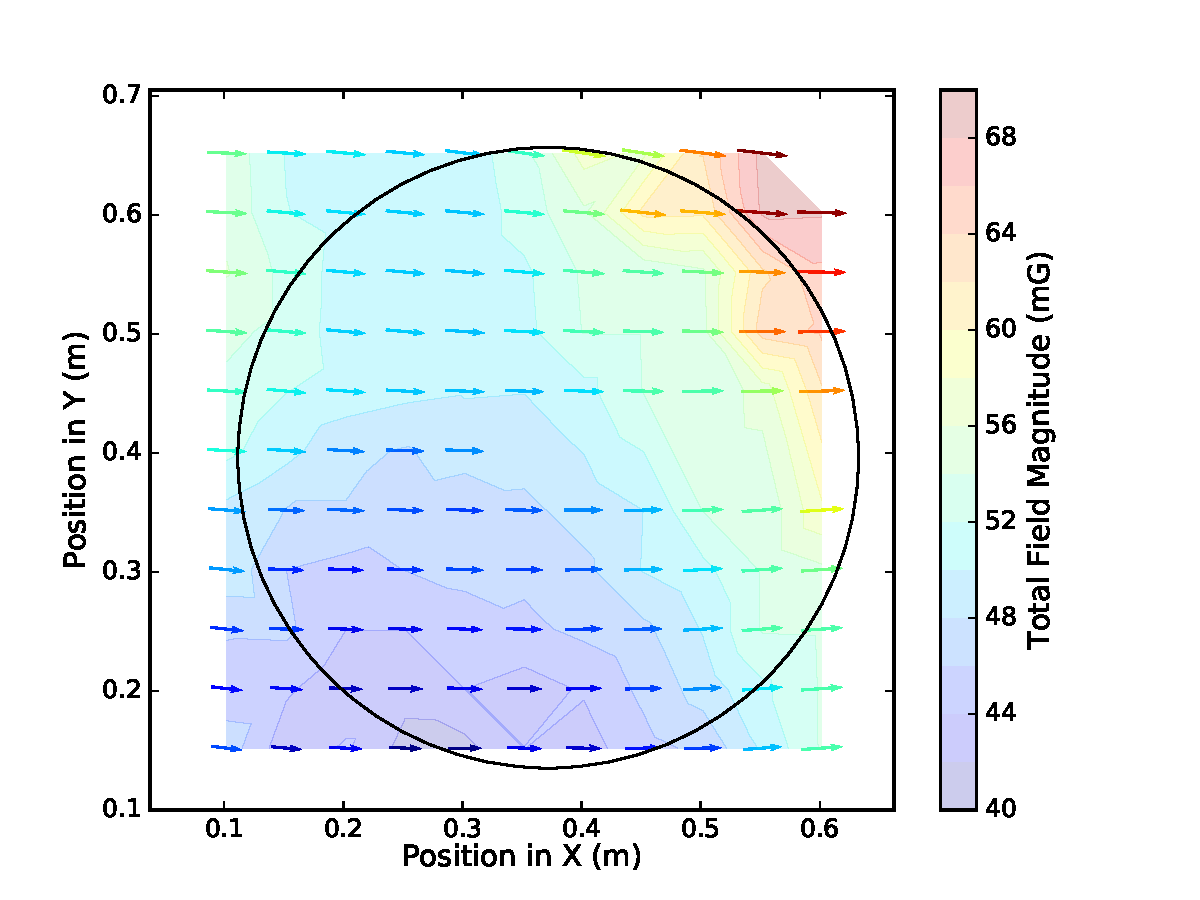
\includegraphics[width=0.5\textwidth]{bfield_rep_Bx50_z700_2_vec.pdf}
    }\\
    \vspace{-3 mm}
    \subfloat[Trial 1: x-component of magnetic field\label{fig:bfield_rep_Bx50_1_x}]{
      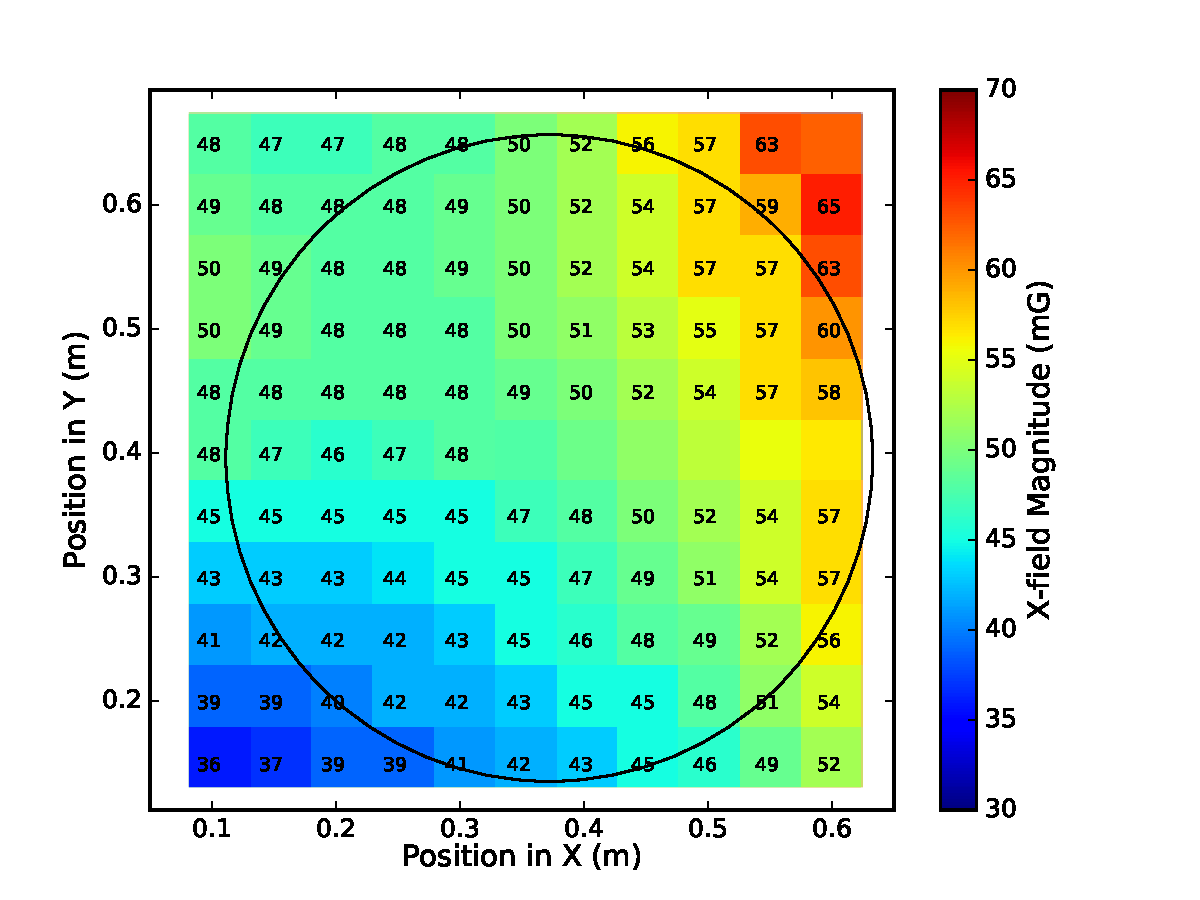
\includegraphics[width=0.5\textwidth]{bfield_rep_Bx50_z700_1_x.pdf}
    }
    \subfloat[Trial 2: x-component of magnetic field\label{fig:bfield_rep_Bx50_2_x}]{
      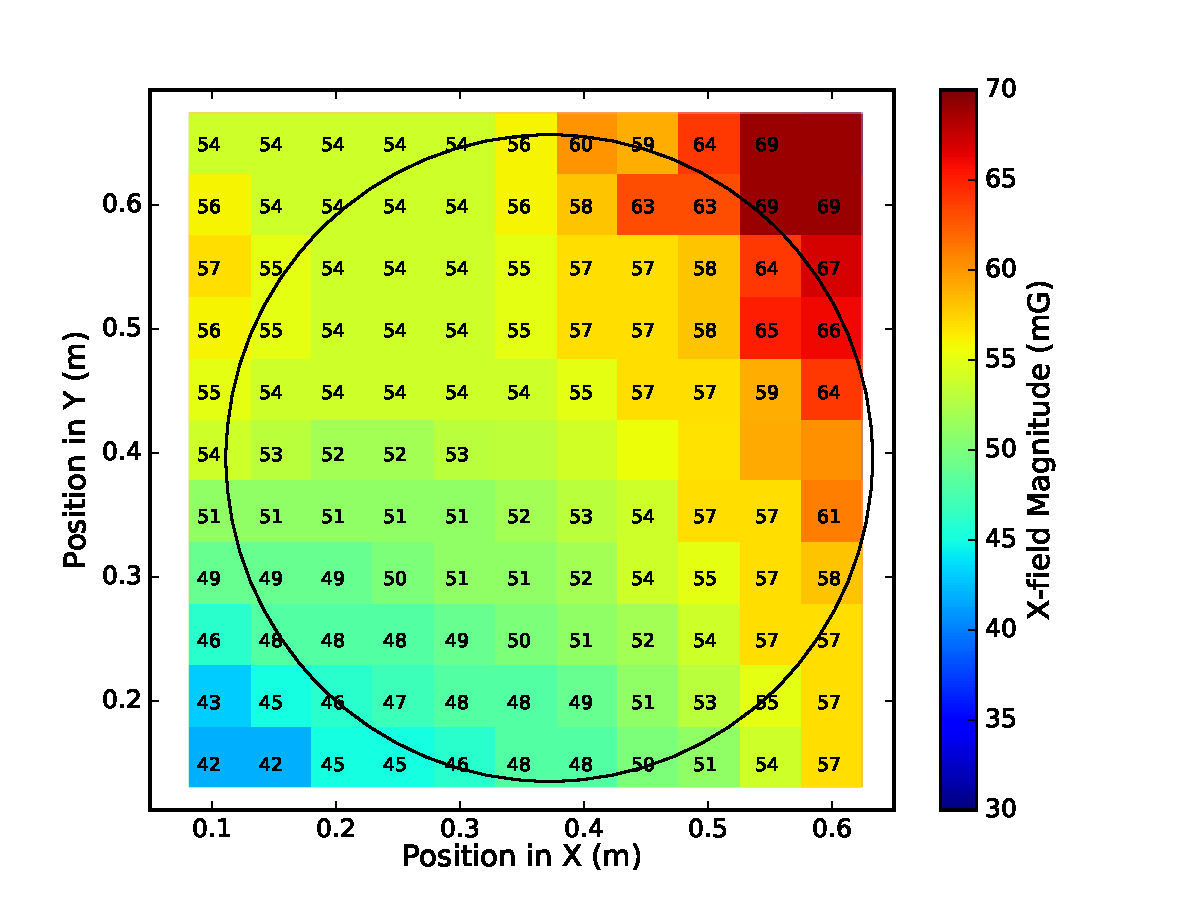
\includegraphics[width=0.5\textwidth]{bfield_rep_Bx50_z700_2_x.pdf}
    }
  \caption{Plots of magnetic field with an offset of 50 mG in the x-direction.}
  \label{fig:bfield_rep_Bx50}
  \end{center}
\end{figure}
%
%
\begin{figure}[h!]
  \begin{center}
    \subfloat[Trial 1: magnetic field magnitude and vector field\label{fig:bfield_rep_By150_1_vec}]{
      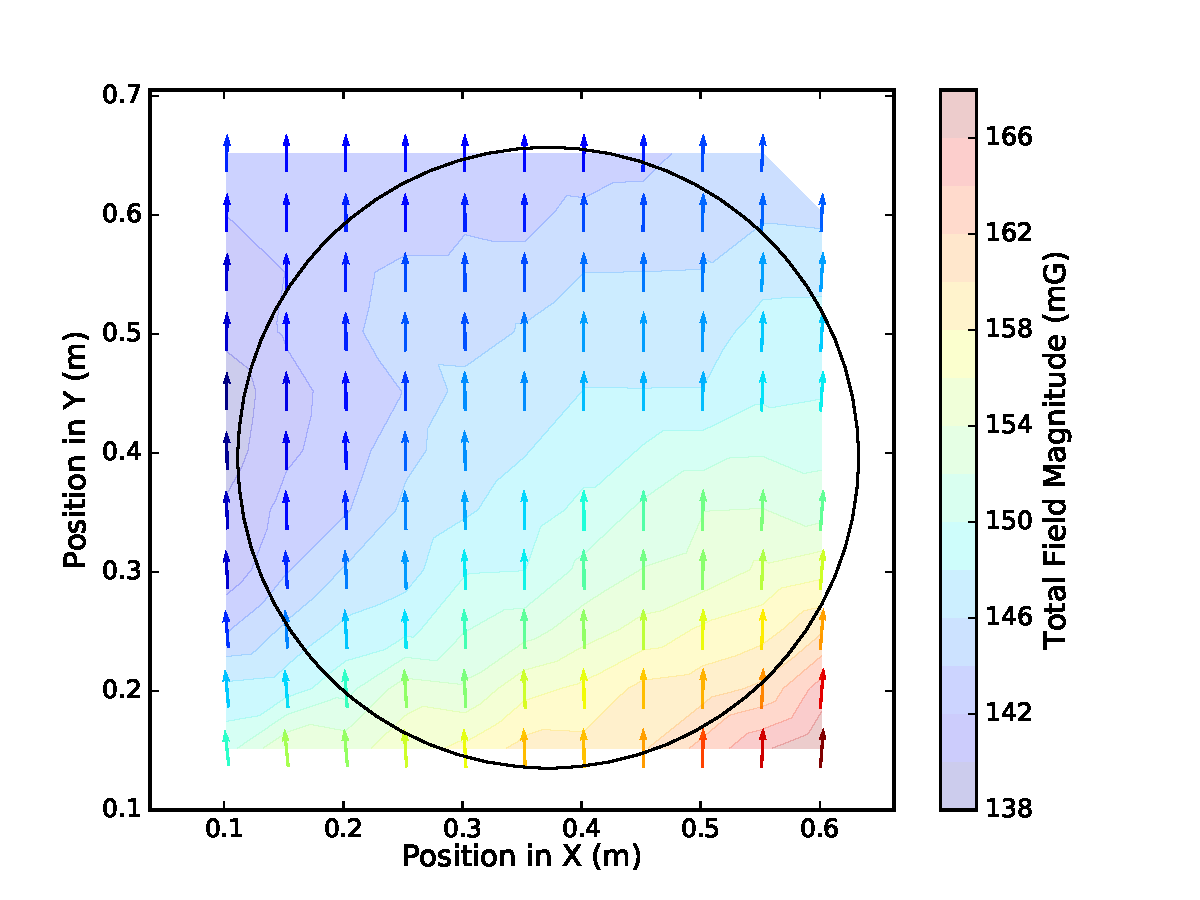
\includegraphics[width=0.5\textwidth]{bfield_rep_By150_z700_1_vec.pdf}
    }
    \subfloat[Trial 2: magnetic field magnitude and vector field\label{fig:bfield_rep_By150_2_vec}]{
      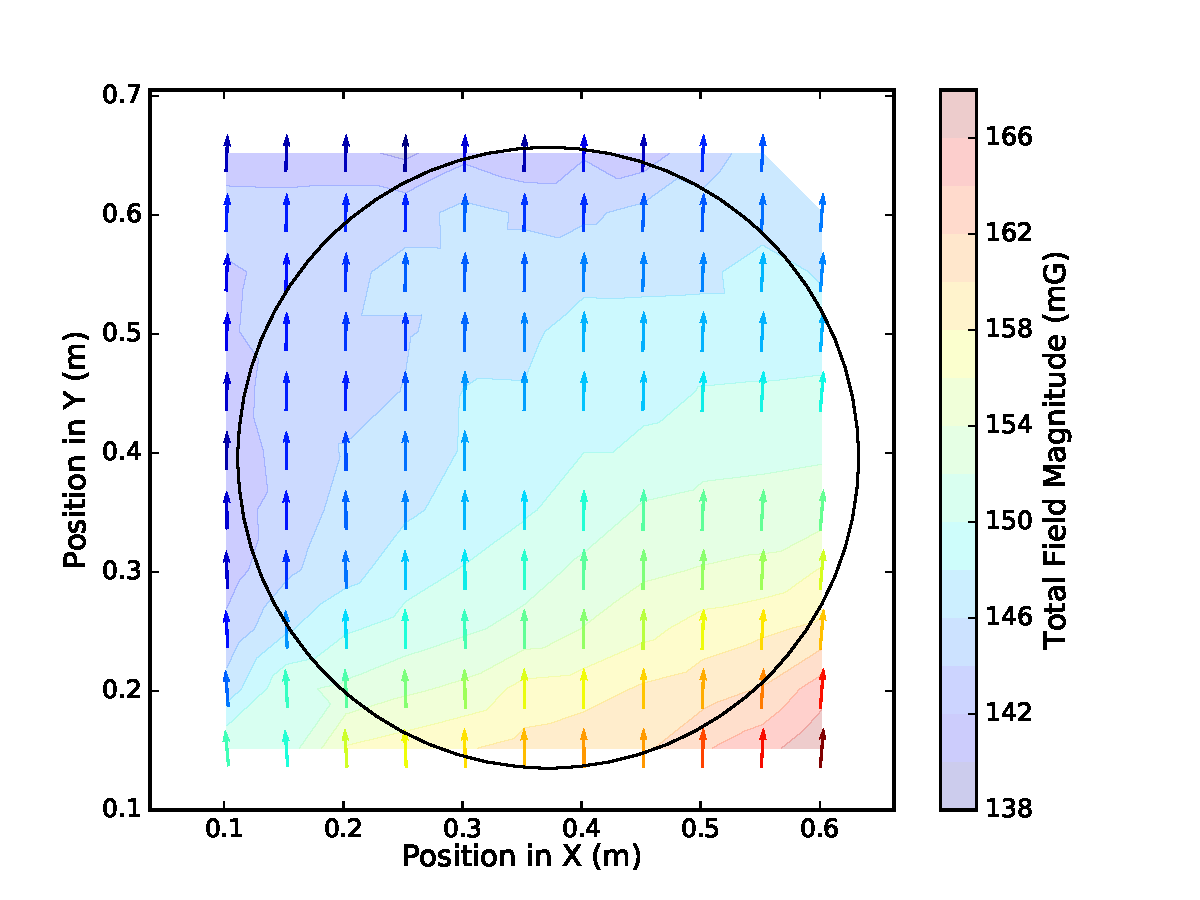
\includegraphics[width=0.5\textwidth]{bfield_rep_By150_z700_2_vec.pdf}
    }\\
    \vspace{-3 mm}
    \subfloat[Trial 1: y-component of magnetic field\label{fig:bfield_rep_By150_1_y}]{
      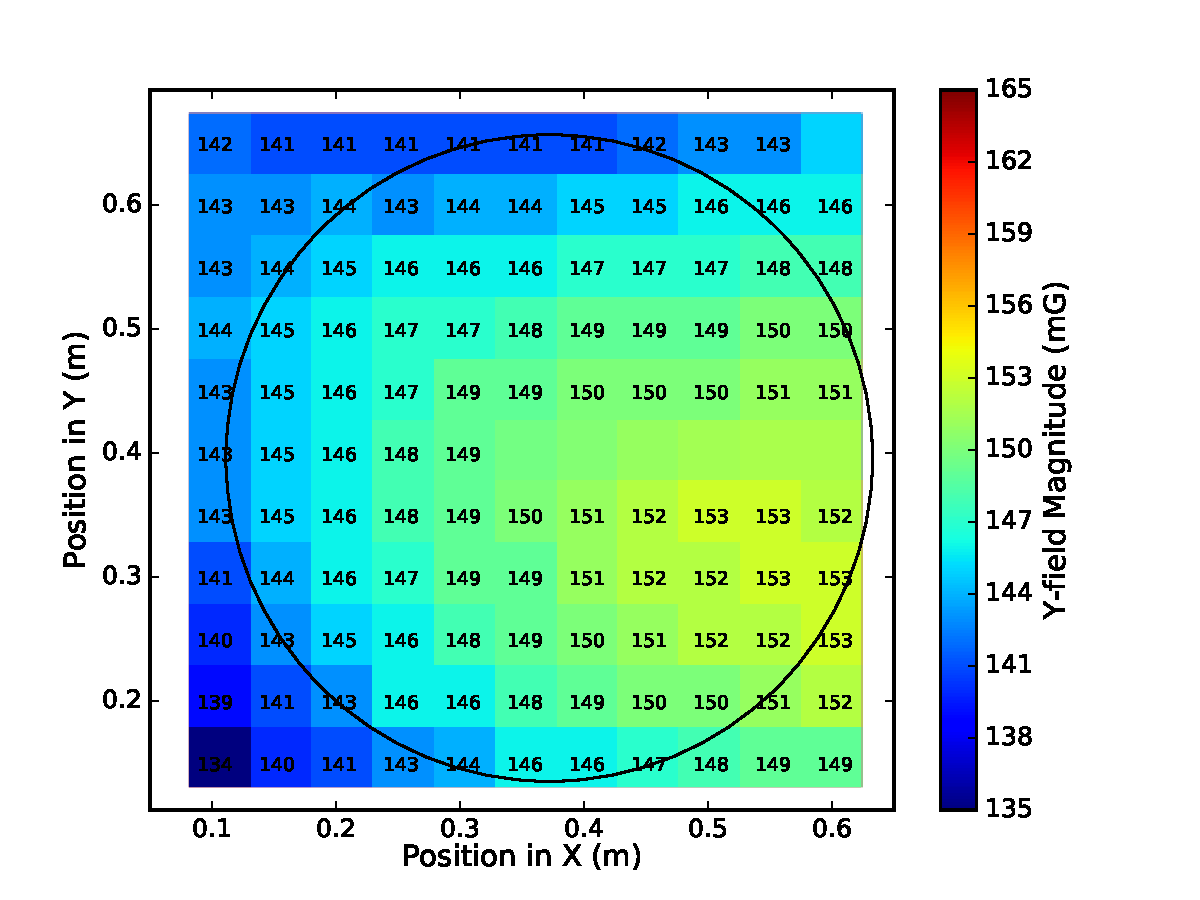
\includegraphics[width=0.5\textwidth]{bfield_rep_By150_z700_1_y.pdf}
    }
    \subfloat[Trial 2: y-component of magnetic field\label{fig:bfield_rep_By150_2_y}]{
      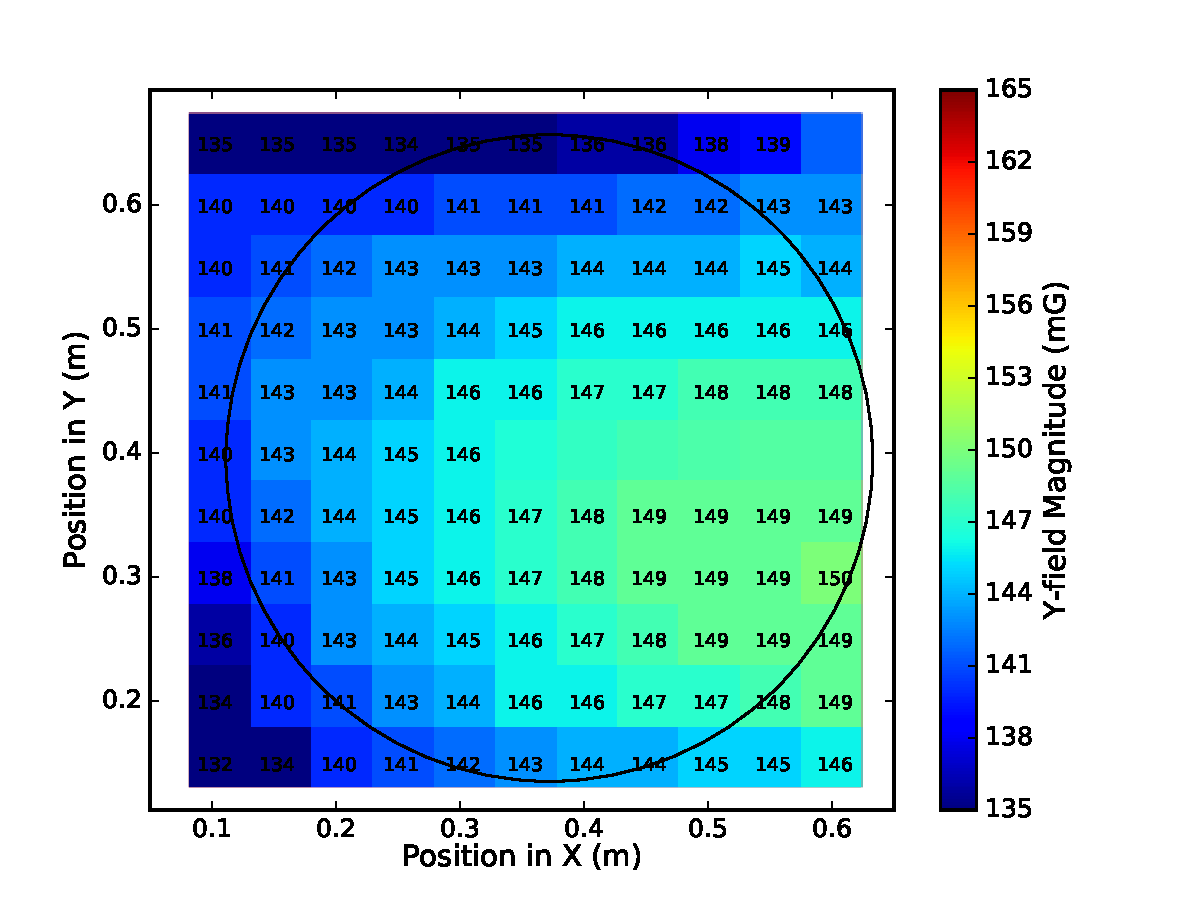
\includegraphics[width=0.5\textwidth]{bfield_rep_By150_z700_2_y.pdf}
    }
  \caption{Plots of magnetic field with an offset of 150 mG in the y-direction.}
  \label{fig:bfield_rep_By150}
  \end{center}
\end{figure}
%
%
\begin{figure}[h!]
  \begin{center}
    \subfloat[Trial 1: magnetic field magnitude and vector field\label{fig:bfield_rep_Bzn100_1_vec}]{
      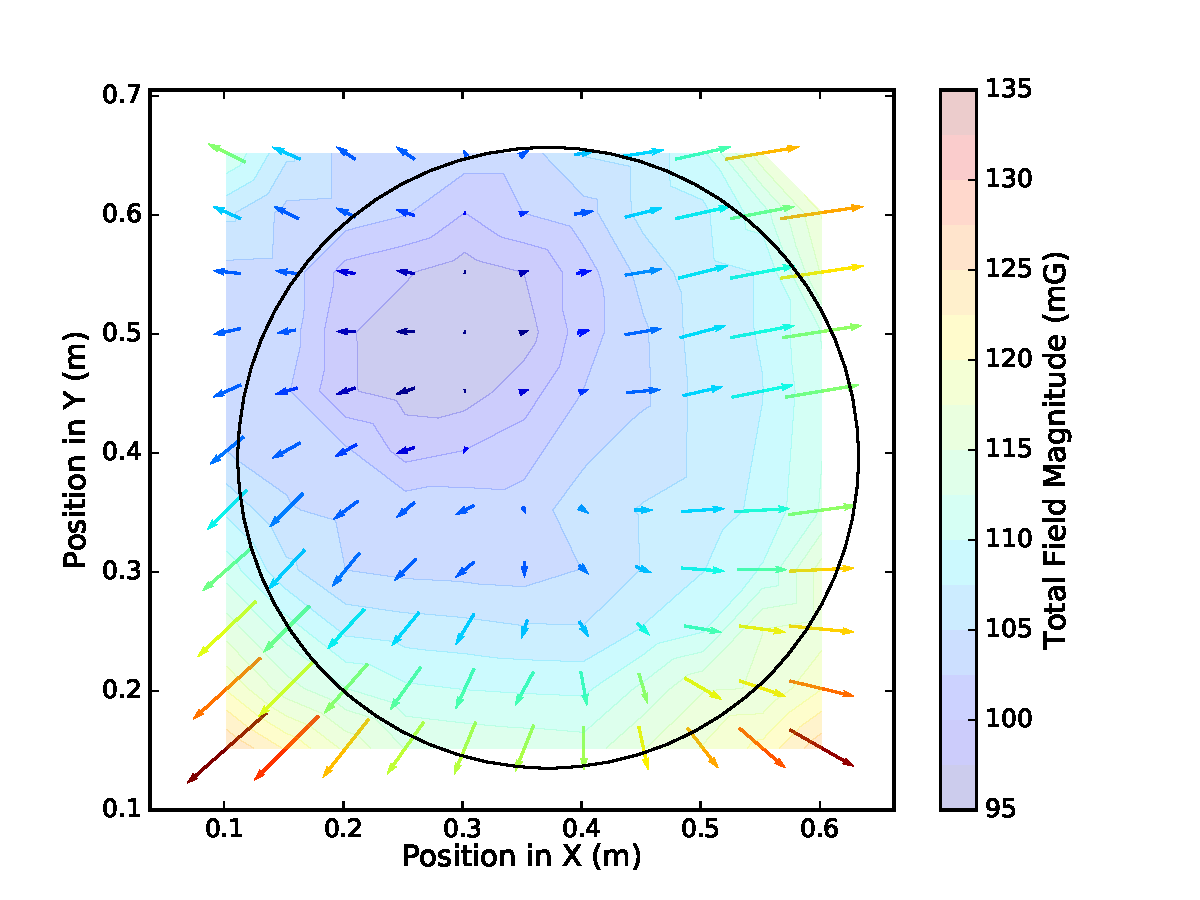
\includegraphics[width=0.5\textwidth]{bfield_rep_Bzn100_z700_1_vec.pdf}
    }
    \subfloat[Trial 2: magnetic field magnitude and vector field\label{fig:bfield_rep_Bzn100_2_vec}]{
      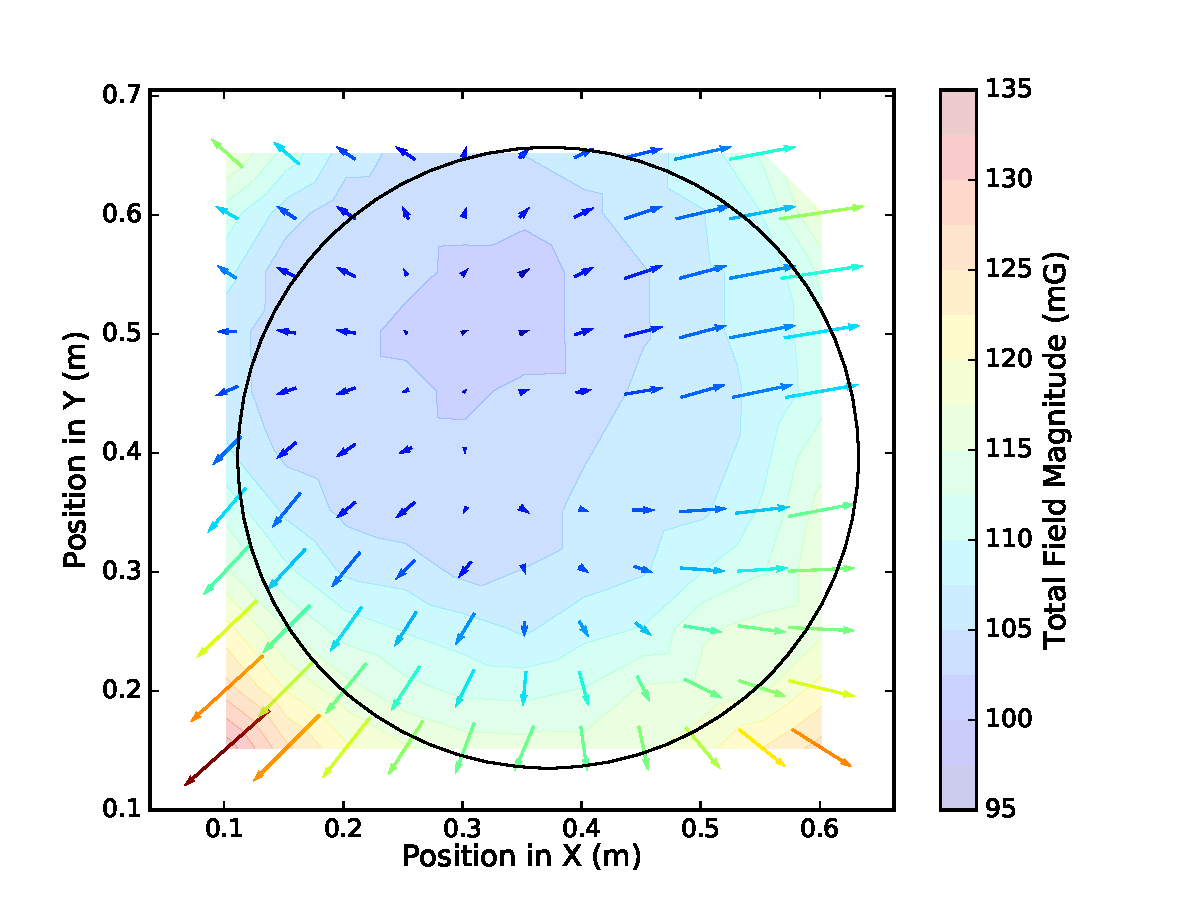
\includegraphics[width=0.5\textwidth]{bfield_rep_Bzn100_z700_2_vec.pdf}
    }\\
    \vspace{-3 mm}
    \subfloat[Trial 1: z-component of magnetic field\label{fig:bfield_rep_Bzn100_1_z}]{
      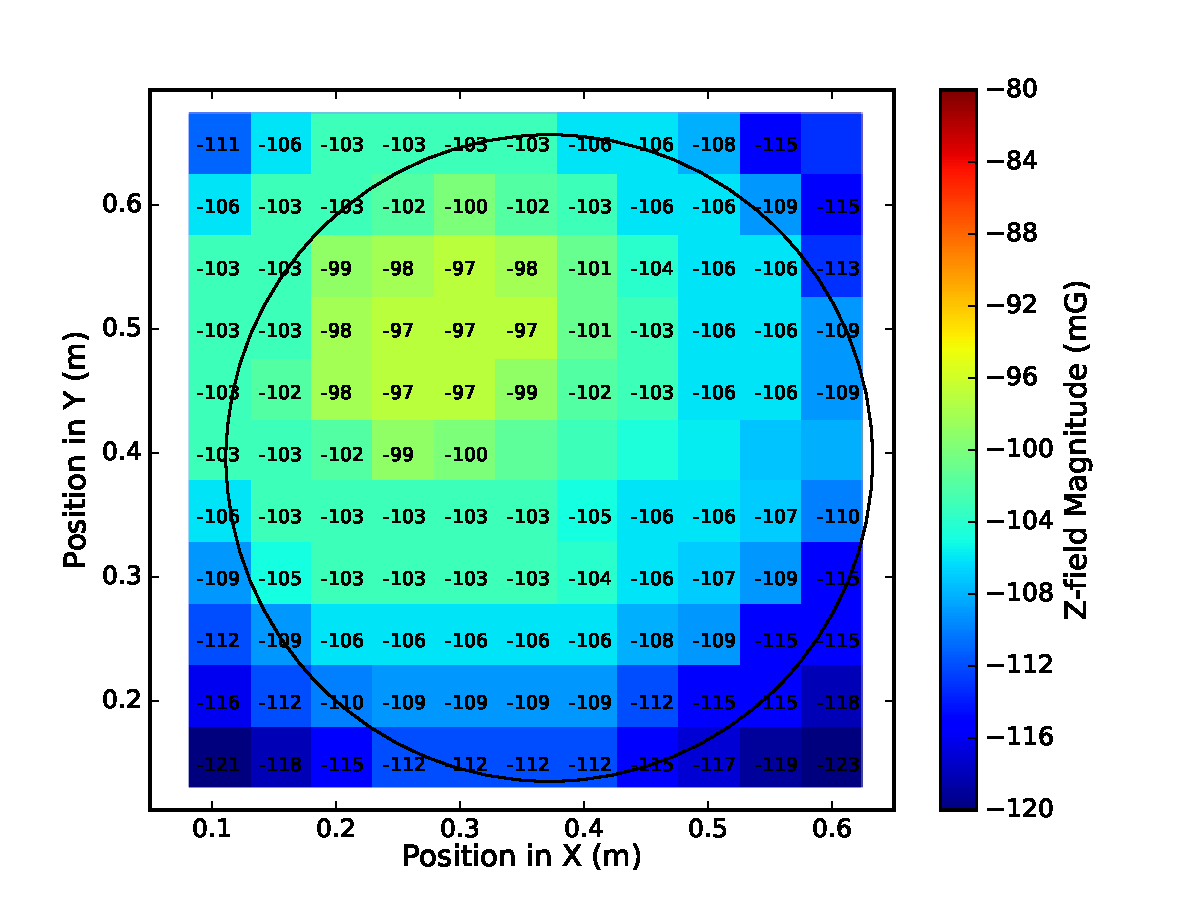
\includegraphics[width=0.5\textwidth]{bfield_rep_Bzn100_z700_1_z.pdf}
    }
    \subfloat[Trial 2: z-component of magnetic field\label{fig:bfield_rep_Bzn100_2_z}]{
      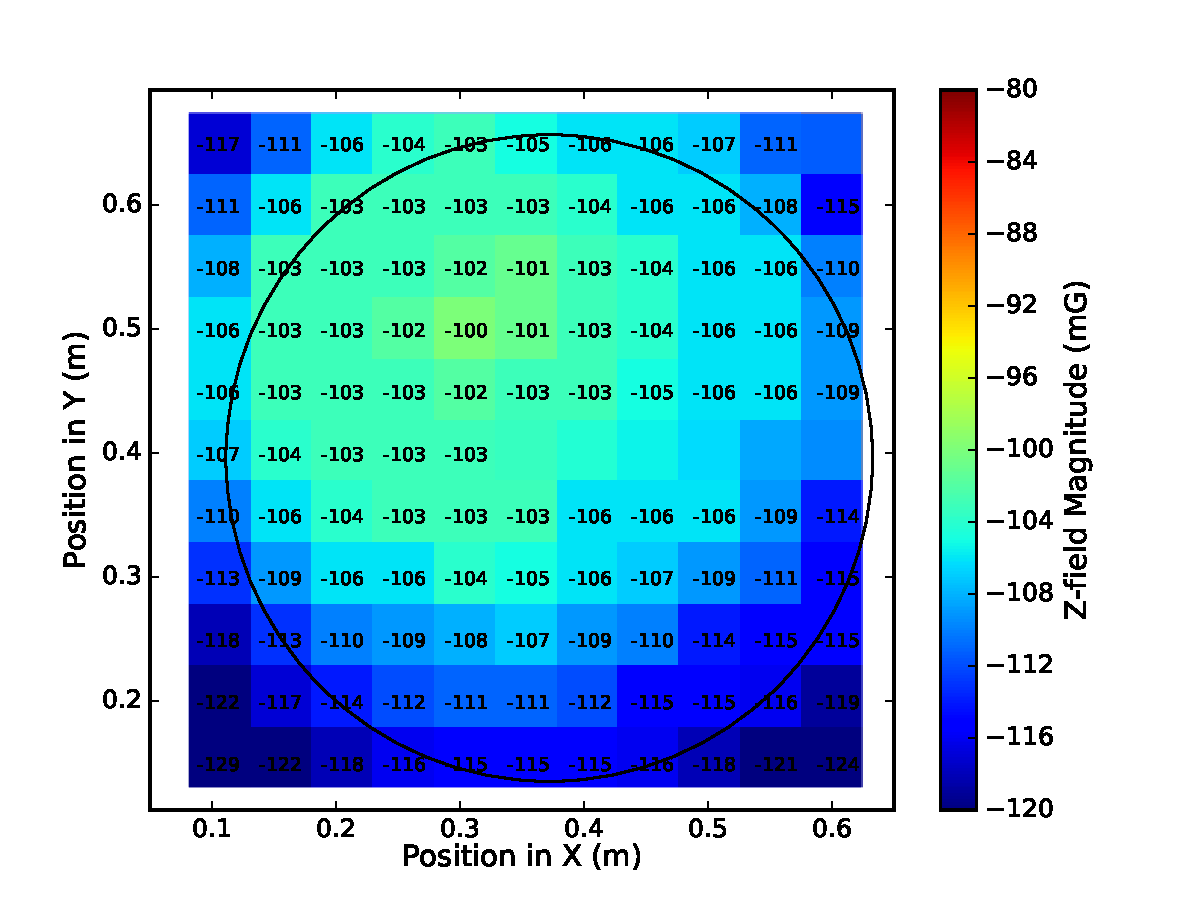
\includegraphics[width=0.5\textwidth]{bfield_rep_Bzn100_z700_2_z.pdf}
    }
  \caption{Plots of magnetic field with an offset of -100 mG in the z-direction.}
  \label{fig:bfield_rep_Bzn100}
  \end{center}
\end{figure}
%
\newpage
